\documentclass[14pt]{beamer}

\usepackage[utf8]{inputenc}
\usepackage[czech]{babel}

\usepackage{enumerate}
\usepackage[shortlabels]{enumitem}
\usepackage{pifont}

%\usetheme{Warsaw}
\title{Animace postav}
\author{Tomáš Maršáelek}
\date{\today}

\begin{document}

\begin{frame}
\titlepage
\end{frame}

\begin{frame}{2D animace postav}
\begin{columns}[c]
\column{.4\textwidth}
\begin{itemize}[label=-]
	\item<1-> Disney
	\item<2-> Cartoon
	\item<3-> Anime
\end{itemize}
\column{.4\textwidth}
\centering
\only<1->{
\includegraphics[height=.4\textheight]{mickey-mouse1.jpg}}
\end{columns}

\begin{columns}[c]
\column{.4\textwidth}
\centering
\only<3->{
\includegraphics[height=.4\textheight]{anime.png}}
\column{.4\textwidth}
\hfill
\only<2->{
\includegraphics[height=.4\textheight]{spiderman.jpg}}
\end{columns}

\end{frame}

\begin{frame}{3D animace postav}
\begin{itemize}
	\item MoCap
	\item Rotoskopie
	\item Ruční animace
\end{itemize}
\end{frame}

\begin{frame}{Motion Capture (MoCap)}
\only<1>{
	\begin{columns}[c]
	\column{.5\textwidth}
	\begin{itemize}[label=+]
		\item rychlejší, realističtější animace
	\end{itemize}
	\begin{itemize}[label=-]
		\item pořizovací náklady HW a SW
		\item pouze pro fyzicky reálný pohyb
		\item pozor na neproporcionální postavy
	\end{itemize}

	\column{.5\textwidth}
	\hfill
	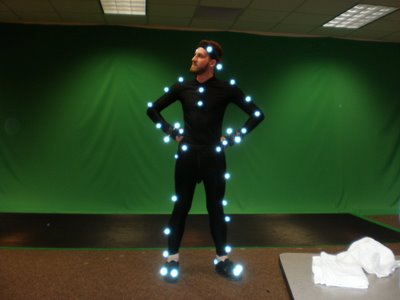
\includegraphics[height=.45\textheight]{mocap1.jpg}
	\end{columns}
}

\only<2>{
	\begin{center}
	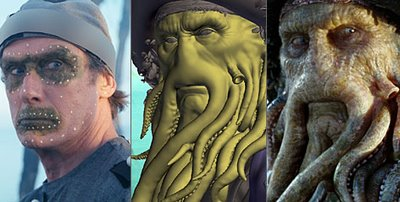
\includegraphics[width=.95\textwidth]{mocap2.jpg}
	\end{center}
}
\end{frame}

\begin{frame}{Rotoskopie}
\begin{itemize}[label=-]
	\item Animace přes nahraný video záznam
	\item pro 2D i 3D
	\item pro 3D animaci stačí rotoskopovat pár snímků a dointerpolovat
\end{itemize}
\end{frame}

\begin{frame}{Ruční animace}
\begin{itemize}[label=-]
	\item Model
	\item Armatura
	\item Deformace
	\item Omezení
	\item Funkce (na prsty, obličej, atd.)
\end{itemize}
\end{frame}

\begin{frame}{Dodání života postavám}
\begin{itemize}[label=-]
	\item 12 základních principů animace
	\item animátoři pro Disney Ollie Johnston a Frank Thomas 
	\item The Illusion of Life - \uv{Bible animace}
	\item vytvořit iluzi, aby se postavy řídily zákony fyziky
	\item důraz na dojem z postavy
\end{itemize}
\end{frame}

\begin{frame}{12 principů}
\only<1>{
	\begin{enumerate}[1.]
		\item Zplácnutí a roztáhnutí (Squash and stretch)
		\item Očekávání (anticipation)
		\item Režie (staging)
		\item Animování přímo proti animování klíčkových pozic
		\item Setrvačnost a překrývající se akce (Follow through and overlapping action)
		\item Pomalu před akcí a pomalu po akci (Slow in and slow out)
	\end{enumerate}
}
\only<2>{
	\begin{enumerate}[1.]
		\setcounter{enumi}{6}
		\item Oblouky (Arcs)
		\item Druhotná akce (Secondary action)
		\item Časování (Timing)
		\item Přehánění (Exaggeration)
		\item Dovednosti v rýsování (Solid drawing)
		\item Charisma postav (Appeal)
	\end{enumerate}
}
\end{frame}

\begin{frame}{Zdroje pro zdokonalení se v animaci}
\begin{columns}[c]
\column{.4\textwidth}
\only<1>{Illusion of Life - 12 základních principů animace}
\only<2>{Animation Mentor}
\only<3>{Jeff Lew}

\column{.6\textwidth}
\only<1>{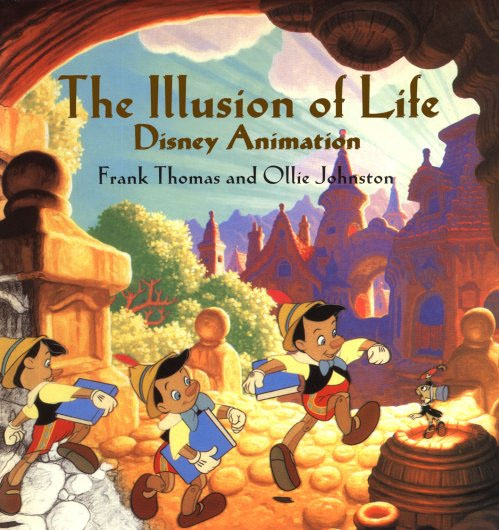
\includegraphics[height=.8\textheight]{Book_the_illusion_of_life.jpg}}
\end{columns}

\only<3>{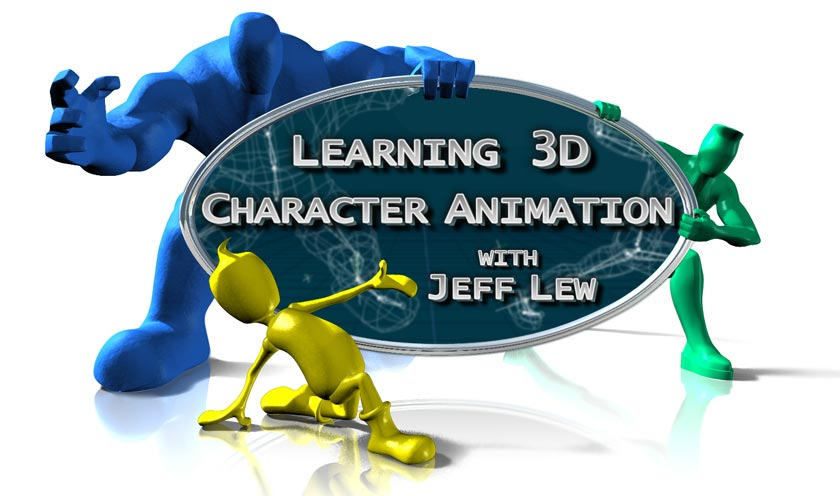
\includegraphics[width=.95\textwidth]{jefflew1.jpg}}
\end{frame}

\end{document}
